\documentclass{article}

\usepackage[utf8]{inputenc}
\usepackage{url}
\usepackage{amsmath}
\usepackage{graphicx}
\usepackage{geometry}
\usepackage{ragged2e}

\geometry{
a4paper,
left=30mm,
right=20mm,
top=30mm,
bottom=20mm,
}

\renewcommand{\figurename}{Fig.}

\usepackage[backend=bibtex,style=authoryear]{biblatex}
\renewcommand*{\nameyeardelim}{\addcolon\space}

\newlength{\bibparskip}\setlength{\bibparskip}{0pt}
\let\oldthebibliography\thebibliography
\renewcommand\thebibliography[1]{%
  \oldthebibliography{#1}%
  \setlength{\parskip}{\bibitemsep}%
  \setlength{\itemsep}{\bibparskip}%
}

\setlength{\bibitemsep}{1.2\baselineskip}

\renewcommand{\contentsname}{Sumário}
\renewcommand{\listfigurename}{Figuras}
\begin{document}

	\pagenumbering{gobble}
	\begin{center}

		{\LARGE Universidade Federal de Santa Catarina \par}
		\vspace {2cm}
		
		Ciências da Computação
		\vspace{2cm}

		Luca Fachini Campelli
		\vspace {4cm}

		\textbf{DESENVOLVIMENTO DE UMA APLICAÇÃO PARA COLETA DE DADOS \\
				E EMISSÃO DE PASSAPORTES ELETRÔNICOS NA PLATAFORMA JAVACARD}
		\vspace {10cm}
		
		Florianópolis/SC \\

		2018
	\end{center}

	\newpage
	\begin{center}
		Luca Fachini Campelli
		\vspace{2cm}
		
		\textbf{\large DESENVOLVIMENTO DE UMA APLICAÇÃO PARA COLETA DE DADOS \\
				E EMISSÃO DE PASSAPORTES ELETRÔNICOS NA PLATAFORMA JAVACARD}
		\vspace{2cm}

		\hfill \textbf{Trabalho de Conclusão de Curso \\}
		\hfill \textbf{para a graduação no curso de\\}
		\hfill \textbf{Ciências \hspace{18pt} da \hspace{18pt} Computação \\}
		\hfill \textbf{UFSC  \hspace{60pt}}

		\vspace{1cm}

		\hfill Florianópolis, 2018

	\end{center}

	\newpage

	\paragraph{\large Resumo (Melhorar)}
		\begin{justify}
			\hspace{2cm} Foi desenvolvido um software para computador capaz de coletar as informações do usuário, e emitir um passaporte eletrônico em um Javacard que segue o padrão ICAO 9303. Este cartão é munido de todas as informações necessárias para a verificação da identidade do usuário, incluindo informações biométricas como identificação facial, e digitais, juntamente com todos os mecanismos de segurança descritos pelo documento ICAO 9303.
	
	\vspace*{10px}
Palavras-chave: Javacard, Passaporte,JMRTD, Segurança, Passaporte-Eletrônico, e-Passport, SmartCard, JCOP
		\end{justify}


	\paragraph{\large Abstract}
		\begin{justify}

			\hspace{2cm} A computer software was developed capable of collecting user information, and emiting an electronic passport on a Javacard that follows the ICAO 9303 standard. This card posesses all required information to verify the user's identity, including biometrics such as face recognition and fingerprints, together with all security mecanisms described in the ICAO 9303 document.

	\vspace*{10px}
Key-Words: Javacard, Passaport,JMRTD, Security, Electronic-Passport, e-Passport, SmartCard, JCOP

		\end{justify}
	
	\newpage

	\tableofcontents
	\listoffigures
	\newpage

	\pagenumbering{arabic}

	\section{Introdução}
		\begin{justify}
			
			\hspace{2cm} Quando começaram a ser utilizados, os passaportes funcionavam apenas por meio físico, na forma de uma caderneta ou documento escrito, com todas as informações sendo verificadas manualmente, comparando as informações com o outros papéis, o que abria brechas para a falsificação. Conforme o documento foi evoluindo, até se tornar a caderneta que conhecemos hoje, várias formas de prevenir falsificações como marcas d’água, padrões de impressão e manufatura do papel foram utilizadas, porém a inovação mais impactante e discutida foi a inserção de um chip eletrônico dentro do passaporte \parencite{PASSPORTWIKI}. Embora várias informações possam ainda ser verificadas visualmente mais ainda podem ser verificadas por meio deste chip interno do passaporte, e mais rapidamente, permitindo até que a aferição do passaporte seja automatizada. Este chip pode guardar as informações biométricas do dono, junto com as informações visuais, e ainda mais importante, possuindo diversos protocolos de segurança para garantir a autenticidade dos dados conferidos \parencite{HOWPASSPORT}.\\
			\hspace*{2cm} Diversos softwares existem para a leitura de passportes e, daqueles escritos em Java, em sua maioria se utilizam da biblioteca JMRTD\parencite{JMRTD} como base para seu funcionamento, mas não foi possível encontrar o software utilizado por aeroportos para a verificação de passaportes. Sendo assim, seria possível emitir um passaporte na plataforma javacard, utilizando bibliotecas open-source, que seja equivalente ao passaporte utilizado hoje em dia?

			
		\end{justify}

	\subsection{Objetivos}
		\begin{justify}
				
			\hspace{2cm}O objetivo principal é a criação do sistema de coleta de dados e emissão de um passaporte eletrônico em um cartão Javacard, onde os dados sejam armazenados depois possam ser extraídos e validados em qualquer tipo de máquina que possua este sistema.\\
			\hspace*{2cm}Desta forma, alguns requisitos são propostos para que o objetivo se dê por alcançado:\\
				\hspace*{3cm}1.O sistema deve coletr os dados básicos do usuário\\
				\hspace*{3cm}2.O sistema deve tirar a foto do usuário e extrair dela os dados para o reconhecimento facial.\\
				\hspace*{3cm}3.O sistema deve coletar os dados biométricos como digital e íris.\\
				\hspace*{3cm}4.Ter o cartão preenchido e que cumpra as especificações do padrão ICAO9303.\\
				\hspace*{3cm}5.O cartão deve ser equivalente a um passaporte oficial, na questão de sua estrutura interna e dados armazenados\\
			\hspace*{2cm}Ao final do projeto espera-se ter concluído a criação de um sistema que colete os dados do usuário, armazenando-os no cartão, conforme as especificações ditadas no padrão ICAO9303

			
		\end{justify}

	\subsection{Trabalhos Correlatos e Revisão Bibliográfica} Falar um paragrafo mais ou menos sobre cada um, pros contras pq o seu será melhor?
		\begin{justify}
			Parametrizar o método de busca para deixar mais forte esta seção. Com qual query de busca que se chegou o resultado, qual foi a extensão da busca.\\
			\hspace{2cm} Várias bibliotecas e aplicativos funcionais existem, que fazem possível a leitura de passaportes eletrônicos, ou por via de chips de contato ou RFID, escritos em várias linguagens de programação. Muitos poucos permitem a emissão e personalização destes passaportes. Para a linguagem Java, vários se utilizam também da biblioteca JMRTD. \\
			\hspace*{2cm}A pesquisa foi efetuada utilizando-se a plataforma de busca Google, com as seguintes pesquisas: "e-passport reader python", "e-passport reader java", "e-passport reader c++", "e-passport creation", "passport creation python", "passport creation java", sendo analisada toda a primeira e segunda páginas da busca, e os que mais se destacaram foram:\\
			\hspace*{2cm}\textbf{pypassport} - É uma API desenvolvida em python que permite a interação com passaportes eletrônicos. Ela permite a leitura das informações e execução dos protocolos BAC, PA e AA. Ele também permite a criação do conteúdo de um passaporte eletrônico, porém não permite sua personalização.\parencite{PYPASSPORT}\\
			\hspace*{2cm}\textbf{readid} - Um aplicativo android desenvolvido pela empresa InnoValor para leitura de passaportes eletrônicos em smartphones com capacidade NFC. Não provê funcões de personalização nem criação de passaportes, mas "por enquanto não se sabe se faz os protocolos basicos de segurança"\parencite{INNOVALOR}\\
			\hspace*{2cm}\textbf{e-passport NFC reader} - Um aplicativo android desenvolvido para leitura de passaportes eletrônicos. Se utiliza da biblioteca JMRTD para seu funcionamento, e execução do protocolo BAC. Como é um aplicativo mobile, não permite a personalização de passaportes.\parencite{TANANAEV}\\
			\hspace*{2cm}\textbf{epassport reader} - Um programa desenvolvido em Java para a leitura de passaportes. Se utiliza da biblioteca JMRTD para seu funcionamento e execução do protocolo BAC, porém não permite a personalização de passaportes.\parencite{GLAMDRING}\\

		\end{justify}

	\section {Fundamentações teóricas e práticas}
		\subsection{Criptografia Simétrica e Assimétrica}
			\begin{justify}
			

	 			\hspace{2cm} É possível cifrar a informação para que apenas quem possua a chave da cifra possa acessa-la. O ato de embaralhar o significado da mensagem se chama cifrar, e o inverso, decifrar. Para tal, utiliza-se algum tipo de algoritmo que, em conjunto com uma chave, seja capaz de mascarar a informação original e que seja reversível, para que com o uso da chave, se possa desfazer a criptografia e acessar o conteúdo original da mensagem. Nesta área existem dois tipos de protocolos para cifrar mensagens: a criptografia Simétrica e a Assimétrica. \\
				\hspace*{2cm}Na criptografia simétrica, uma única chave é utilizada por ambas as partes, para cifrar e decifrar a mensagem. Na criptografia assimétrica, são utilizadas duas chaves distintas, uma pública e uma privada. Ambas podem ser usadas para cifrar, porém o que uma cifrar, somente poderá ser decifrado pela outra. Devido às dificuldades de se utilizar este protocolo ele é mais utilizado para certificações digitais.
					
			\end{justify}

		\subsection{Função Hash - SHA}
			\begin{justify}
			

				\hspace{2cm} Esta função é amplamente utilizada para garantia de consistência tanto em criptografia quanto em várias outras áreas. Ela funciona embaralhando os bits de uma mensagem à um ponto que seja impossível inverter o processo. Ela aceita uma mensagem de qualquer tamanho, porém sempre retornará uma cadeia de bytes de tamanho fixo, não importando qual seja a entrada. Porém a maior característica desta função está no fato de que para duas entradas distintas x e y quaisquer, o resultado da função sempre será diferente para as duas. Desta forma, é possível se confirmar a integridade de uma mensagem, aplicando a função hash sobre ela antes de ser enviada, e depois de recebida, comparando a hash da mensagem com a hash recebida, pois se a mensagem foi alterada, por menor que seja a alteração, os dois resultados da função serão completamente diferentes. O algoritmo mais utilizado para esta função é o SHA 2 - Secure Hash Algorithm 2(Algoritmo de Hash Seguro 2), projetado pela NSA, e possui seis versões diferentes, onde a mudança principal está no número de bits que eles retornam: SHA-224, SHA-256, SHA-384, SHA-512, SHA-512/224, SHA-512/256. 
			
			\end{justify}

		\subsection{Assinaturas Digitais}
			\begin{justify}
			

				\hspace{2cm}A confiança entre duas partes de uma troca de mensagens pode não ser suficiente para que informação sensível seja transferida. Uma parte “A” pode forjar uma mensagem alegando ter sido enviada pela parte “B”, ou “B” pode simplesmente negar ter enviado qualquer mensagem, mesmo que o tenha. Desta forma, um meio de proteger âmbas as partes contra fraude mútua são as assinaturas digitais.\\
				\hspace*{2cm}Uma assinatura digital consiste normalmente da própria mensagem "M", passada pela função hash e cifrada com a chave privada do remetente, concatenada ao fim da mensagem. Ao ser recebida esta assinatura pode ser verificada, removendo-a da mensagem, decifrando-a com a chave pública do remetente e comparando-a com a hash da mensagem recebida. Sendo assim duas afirmações podem ser concluídas: apenas o remetente pode ter enviado a mensagem, pois apenas a sua chave privada pode ser decifrada com sua chave pública, e a mensagem não foi alterada durante seu trajeto, pois as hash's coicidem.
			
			
			\end{justify}

		\subsection{Certificados Digitais}
			\begin{justify}
			
				
					\hspace{2cm}Certificados digitais são documentos eletrônicos que garantem a autenticidade de um certo elemento. Este que pode ser uma entidade, um site da internet ou um terminal de cartões. Um certificado é composto de algumas informações da entidade,  a chave pública da entidade, e uma assinatura digital sobre o certificado. Dependendo do tipo de certificado, esta assinatura adicionada ao final do documento é cifrada ou com a chave privada de quem o criou, denominado de certificado auto-assinado, ou com a chave privada de uma autoridade certificadora (CA - Certificate Authority). \\

			
			\end{justify}

    
	\subsection{O Documento ICAO 9303}
		\begin{justify}
			
				\hspace*{2cm} O documento ICAO 9303 é o documento emitido que regulamenta passaportes eletrônicos, e é o padrão utilizado para toda formatação de passaportes eletrônicos. ICAO é uma sigla para “International Civil Aviation Organization”, que é uma agência especializada das Nações Unidas. Foi estabelecida em 1944 para gerenciar a admnistração e governância da Convenção de Aviação Civil Internacional (Convenção de Chicago). \\
    			\hspace*{2cm} O documento é escrito em 12 partes, cada uma descreve um aspecto sobre como um passaporte eletrônico deve ser desenvolvido, a primeira parte dando uma introdução sobre o as características de um passaporte eletrônico, e definindo siglas e acrônimos para os documentos seguintes.\\
    			\hspace*{2cm} A segunda parte da especificações sobre a segurança física do cartão, desde o design interno, quanto a produção, transporte e criação do cartão. \\
				\hspace*{2cm} A terceira parte especifica as características sobre a apresentação de todos os tipos de passaporte, como fonte, linguagem, campos de preenchimento e representação das informações. \\
				\hspace*{2cm} A quarta parte específica como os dados para passaportes legíveis por máquina, que possuem forma de livreto como são hoje, mostrando dimensões e formatos dos campos, também chamado de tipo TD3. \\
				\hspace*{2cm} A quinta parte especifica como deve ser o layout dos dados para passaportes do tipo cartão plástico impresso, chamado TD1. Este cartão possui uma zona legível por máquina (MRZ), que possui os dados básicos de seu portador, formatados para mais fácil leitura humana e por máquina, impresso em seu exterior junto com todas as outras informações no verso, e uma imagem do portador.\\
				\hspace*{2cm} A sexta parte se assemelha à quinta, pois descreve as características de cartões do tipo TD2, que possuem de diferente do tipo TD1 apenas suas dimensões, tendo todas as informações necessárias em um lado do cartão, permitindo informações opcionais serem adicionadas ao verso.\\
				\hspace*{2cm} A sétima parte se refere à vistos legíveis por máquina. Estes se assemelham aos tipos de passaportes TD1 e TD2, porém possuem as informações referentes aos vistos.\\
				\hspace*{2cm} A oitava parte não foi preenchida ainda, e é mantida reservada para uso futuro.\\
				\hspace*{2cm} A nona parte fala sobre como se deve dispor das informações biométricas do portador do passaporte, formatos e dados, tomando como principal a identificação facial da pessoa, e como identificações secundárias as digitais e íris.\\
				\hspace*{2cm} A décima parte especifica a estrutura logica de dados (LDS) do cartão, e como se deve armazenar os dados biométricos dentro do cartão.\\
				\hspace*{2cm} A décima primeira parte especifica como funcionam os protocolos de segurança necessários à comunicação do cartão e obtenção dos dados biométricos para verificação da identidade da pessoa.\\
				\hspace*{2cm} Por último a décima segunda parte especifica o funcionamento de todas as assinaturas digitais necessárias à certificação do cartão via chaves públicas, e sua infra-estrutura.\\

		\end{justify}

	\subsection{Javacard}
		\begin{justify}
			

				\hspace{2cm} O Javacard é um cartão eletrônico que possui dois componentes principais, Um chip de contato e um processador interno. Este chip de contato se faz presente do lado externo do cartão, da mesma forma que cartões de crédito ou débito modernos, e cuida da comunicação do cartão com a leitora. O processador interno funciona como um computador, ele roda um sistema operacional Java, o que torna este cartão um Javacard. Ele também possui uma memória interna capaz de armazenar dados. O que diferencia este cartão de cartões de crédito por exemplo, é o fato de o cartão possuir um máquina virtual Java (JVM) instalada. A JVM faz possível o cartão possuir aplicativos em sua memória, conhecidos como applets, e dependendo do programa que os acessar, pode escolher qual deles executar. Estes applets são diferentes dos aplicativos Java desenvolvidos para computador, pois devem levar em conta as limitações de processamento e memória dos cartões. Para tal, existe uma biblioteca de desenvolvimento independente conhecida como Java Card Development Kit oferecida pela empresa Oracle, que também disponibiliza o kit de desenvolvimento java convencional. Dentro do cartão, os applets conversam com o terminal por meio de mensagens, chamadas APDU's, que são em sua maioria padronizadas em formatos específicos. O Chip de contato fornece energia e faz a comunicação entre a leitora ou terminal e o processador. Estes cartões possuem diversos mecanismos de segurança embutidos na própria JVM, por exemplo, os aplicativos rodam isolados uns dos outros, portanto os dados de um aplicativo nunca poderão serem lidos por outro. Os cartões também suportam funções de criptografia, que dependem dos aplicativos para serem utilizadas.

			
		\end{justify}


	\subsection{O applet e sua estrutura lógica de dados}
		\begin{justify}

			\hspace{2cm} A biblioteca JMRTD possui consigo um applet a ser instalado e executado no cartão para o funcionamento da biblioteca. Este applet foi feito juntamente com a biblioteca no padrão ICAO9303, portanto ele pode ser lido inclusive por outras bibliotecas que implementem o padrão. Este applet tem como função armazenar todas as informações referentes a um passaporte, e portanto possui uma estrutura de dados lógica interna descrita pelo padrão ICAO9303:\\
			
			\hspace*{1.5cm} DG 1 — Informação da Zona Legível por Máquina\\
			\hspace*{2cm} DG 2 — Características Faciais (Foto)\\
			\hspace*{2cm} DG 3 — Informações de identificação adicionais (Digitais)*\\
			\hspace*{2cm} DG 4 — Informações de identificação adicionais (Iris)*\\
			\hspace*{2cm} DG 5 — Fotografia impressa na frente do cartão*\\
			\hspace*{2cm} DG 6 — Reservado para uso futuro*\\
			\hspace*{2cm} DG 7 — Assinatura escrita digitalizada*\\
			\hspace*{2cm} DG 8 — Características de dados* **\\
			\hspace*{2cm} DG 9 — Características estruturais* **\\
			\hspace*{2cm} DG 10 — Características substanciais*\\
			\hspace*{2cm} DG 11 — Detalhes pessoais adicionais*\\
			\hspace*{2cm} DG 12 — Detalhes do documento adicionais*\\
			\hspace*{2cm} DG 13 — Detalhes opcionais*\\
			\hspace*{2cm} DG 14 — Informações da chave pública para Controle de Acesso Extendido***\\
			\hspace*{2cm} DG 15 — Informações da chave pública para Autenticação Ativa***\\
			\hspace*{2cm} DG 16 — Pessoas para contato*\\

			\hspace*{1.5cm} * - Opcional\\
			\hspace*{2cm} ** - Ainda não definido\\
			\hspace*{2cm} *** - Condicional, apenas se suportado\\
			
			\hspace*{2cm}Além destes existem mais dois arquivos que não armazenam dados do usuário mas sim dados do cartão, estes são: COM e SOD.\\
			\hspace*{2cm} O arquivo COM, ou Arquivo de Cabeçalho e de Presença de Grupos de Dados, possui a função de armazenar a presença dos arquivos de dados, ou seja, quais arquivos estão presentes no cartão, e informações de versionamento do sistema de arquivos do cartão. \\
			\hspace*{2cm} O arquivo SOD, ou Document Security Object - Objeto de Segurança do Documento, possui a função de armazenar o resultado da função hash de cada arquivo, ou seja, no processo de emissão do cartão, cada arquivo é passado também pela função hash, e seu resultado é armazenado dentro do arquivo SOD. Ele também armazena todas as informações de segurança do cartão como os algoritmos utilizados para a função hash e criptografia.\\
			\hspace*{2cm} O cartão possui também uma zona que é ilegível por meios externos, informações sensíveis a criptografia como chaves privadas são armazenadas ali na sua criação, e depois só podem ser lidas e utilizadas pelo próprio cartão.
		\end{justify}

	\subsection{As bibliotecas utilizadas}
		\begin{justify}
			 
		\hspace{2cm}O sistema principal será desenvolvido na linguagem de programação Java, porém algumas das bibliotecas escolhidas foram escritas na linguagem de programação C ou C++ exigindo a utilização da Interface Nativa Java (JNI) para sua utilização.\\
		
        \hspace*{2cm}JMRTD\\
    \hspace*{2cm}Java Machine Readable Travel Documents: é uma biblioteca para a criação, edição, e aferição de passaportes eletônicos escrita na linguagem de programação Java. Ela foi desenvolvida juntamente com a biblioteca Scuba, que a complementa. Ela possui a capacidade de criar, e editar novos passaportes, além que resgatar as informações de um passaporte pronto. \\
        
		\hspace*{2cm}SCUBA\\
    \hspace*{2cm}Smart Card Utilities for Better Access: é uma biblioteca para a comunicação com cartões eletrônicos da plataforma javacard, escrita na linguagem de programação Java. Ela faz a ponte entre o JMRTD e o javacard possuindo a capacidade de transmitir mensagens e prover a comunicação com os cartões.\\
		
        \hspace*{2cm}STASM\\
    \hspace*{2cm}Active Shape Models with STASM: é uma biblioteca de reconhecimento facial escrita na linguagem de progrmação C++. Ela se utiliza de modelos de formas para reconhecer um rosto em uma foto e retirar os pontos de referência do rosto para que depois seja feito o reconhecimento da pessoa, fazendo uso da biblioteca Open-CV. Possui a maioria dos pontos de reconhecimento parecida com o padrão ISO\parencite{ISO}, e foi escolhida por ser de fácil utilização e possuir uma extensa documentação com exemplos mínimos disponíveis, facilitando a sua compreensão, além de ser complementar à biblioteca Open-CV.\\
		
        \hspace*{2cm}LIBFPRINT\\
    \hspace*{2cm}É uma biblioteca de coleção e verificação de digitais biométricas escrita na linguagem de programação C. Ela provê funções para se coletar uma digital e guardá-la como uma imagem, e depois extrair as minutas desta imagem para que se compare com uma digital recém tirada. Foi escolhida por ter uma documentação extensa, exemplos mínimos e ter sido recomendada pelo orientador deste projeto.\\
		
        \hspace*{2cm}OPEN-CV\\
    \hspace*{2cm}Open Source Computer Vision Library: é uma biblioteca para manipulação de imagens e visão computacional escrita na linguagem de programação C++ e Java. Ela possui funcionalidades para conversão de imagens, e acessar a câmera do dispositivo para tirar fotos ou videos. Ela também provê visão computacional, permitindo identificar formas e rostos na imagem. A biblioteca Stasm amplia a funcionalidade para rostos, detectando mais pontos de interesse no rosto da pessoa, e foi escolhida por ser a mais bem recomendada biblioteca de manipulação de imagens e visão computacional, com relação a sua utilização.\\
		
        \hspace*{2cm}EJBCA\\
    \hspace*{2cm}Open Source PKI Certificate Authority: é uma biblioteca para criação e manejo de certificados digitais auto-assinados escrita na linguagem de programação Java. É necessária para o funcionamento da biblioteca JMRTD, para criação dos certificados verificáveis por cartão (CVC), necessários para a execução dos protocolos de segurança do cartão.\\
		
        \hspace*{2cm}BOUNCYCASTLE\\
    \hspace*{2cm}Bouncy Castle Security Provider: é um provedor de segurança, uma biblioteca que possui funções criptograficas e de geração e acordo de chaves para criptografia escrita na linguagem de programação Java. Toda a segurança da biblioteca do JMRTD é feita com ele, portanto por motivos de compatibilidade foi-se utilizado o bouncycastle como provedor para o sistema final.\\

			
		\end{justify}

\subsection{Os protocolos de segurança}
		\begin{justify}
			\hspace{2cm}Para o acesso as informações do cartão diversos protocolos de segurança devem ser efetuados para garantir a troca segura de mensagens entre o terminal e o cartão, e ter a certeza de que o terminal e o cartão não foram adulterados de alguma maneira. Estes protocolos devem ser corretamente configurados durante a criação do cartão para que garantam a segurança das informações que nele estão guardadas. Todos os protocolos estão completamente descritos no documento ICAO 9303 parte 11\\

			\hspace*{2cm} BAC - Basic Access Control - Controle de Acesso Básico\\
			\hspace*{2cm} Antes de fazer qualquer tipo de operação no cartão, deve-se efetuar este protocolo. Ele utiliza as informações do número do documento, data de nascimento e de validade do cartão para criar chaves simétricas seguras para a troca de mensagens entre o terminal e o cartão criando assim um canal seguro de comunicação. Esta informação estará impressa na frente do cartão, e portanto a execução com sucesso deste protocolo não só garante um canal de comunicação seguro, mas também confirma que as informações impressas batem com as armazenadas no cartão.\\
			
			\hspace*{2cm} PA - Passive Authentication - Autenticação Passiva\\
			\hspace*{2cm} Este protocolo faz uso dos arquivos COM e SOD para seu funcionamento. O arquivo SOD armazena a hash de cada Grupo de Dados presente no cartão, e o arquivo COM indica sua presença. Desta forma o protocolo se inicia verificando se para cada arquivo cuja presença esteja indicada em COM, incluindo o próprio arquivo COM, se sua hash coincide com a hash armazenada em SOD. Se todas coincidirem então nenhum arquivo foi alterado desde a fabricação do cartão.\\
			\hspace*{2cm} O segundo passo consiste em utilizar o certificado de assinatura encontrado no SOD, construindo uma corrente de certificação até um certificado assinado por uma CA reconhecida, e garantindo que cada certificado da corrente seja válido. Passados por estes dois passos então se pode confirmar que os dados do cartão são válidos e não foram alterados.\\
			
			\hspace*{2cm} AA - Active Authentication - Autenticação Ativa\\
			\hspace*{2cm} Este protocolo deve ser feito após o PA, pois ele confirma que o SOD foi lido de um cartão com um chip válido. Ele consiste em uma troca de mensagens de desafio-resposta onde a aplicação envia uma mensagem ao cartão e este responde com esta mensagem cifrada pela chave privada do cartão. A aplicação então decifra utilizando a chave pública armazenada no arquivo DG15 e, caso a resposta coincida com a mensagem enviada, então o chip não foi adulterado, já que a chave privada interna do cartão, inacessível externamente, é o par da chave pública gravada no arquivo DG15.\\
			
			\hspace*{2cm} EAC - Extended Access Control - Controle de Acesso Extendido\\
			\hspace*{2cm} Este protocolo deve ser feito após o BAC e é necessário para se obter acesso as biometrias adicionais do cartão. Ele consiste em autenticar o terminal para o cartão, e o cartão para o terminal em duas etapas, utilizando-se de um par de chaves assimétricas. Ao término do protocolo um canal de comunicação de maior segurança entre o cartão e o terminal é gerado, e o acesso às biometrias adicionais é liberado.
			
		\end{justify}

	\section{Desenvolvimento - Reescrever? }
		\begin{justify}
			
		\hspace{2cm}O projeto foi desenvolvido tendo como base o aplicativo JMRTD\parencite{JMRTD}, que engloba uma Biblioteca Java e um Applet, para que seja criado um aplicativo que emita os passaportes, e que possa ser expandido caso haja a necessidade, para englobar mais documentos e não só o passaporte.\\
		\hspace*{2cm}Foi feita uma extensa pesquisa sobre os documentos ICAO 9303\parencite{ICAO}, e a documentação da biblioteca JMRTD para se iniciar o projeto.\\
		\hspace*{2cm}O programa foi desenvolvido com a linguagem de programação Java, utilizando o sistema JNI para a integração de bibliotecas que existem somente em C e C++, e as bibliotecas JMRTD, como a biblioteca principal para a construção do cartão, BouncyCastle\parencite{BOUNCYCASTLE} e EJBCA\parencite{EJBCA} como provedores de segurança e certificação, libfprint\parencite{PRINT} para a coleta das digitais biométricas, Stasm\parencite{STASM} para o reconhecimento facial, e OpenCV\parencite{OPENCV} para processamento de imagem.\\
		\hspace*{2cm}Utilizando uma parte do código da versão 0.4.9 da biblioteca JMRTD, é possível enviar informações para o cartão, desta forma pode-se fácilmente coletar e enviar as informações à respeito do MRZ. A biblioteca OpenCV foi usada para o processamento da foto da pessoa, e possui funções para tirar a foto com a camera da máquina. Com a biblioteca Stasm, se pode retirar os pontos faciais da pessoa, e depois tratá-los para se adequarem ao padrão ICAO. Foi necessário utilizar a API nativa do java para integrar as bibliotecas Stasm e libfprint ao projeto, pois elas existem apenas em C. Com a biblioteca libfprint foi possível a extração da digital para sua inserção.\\
		\hspace*{2cm}Durante o desenvolvimento, alguns pontos chave tiveram uma quantidade de esforço maior para serem desenvolvidos. Para a captura de digitais, e leitura facial, as bibliotecas libfprint e Stasm, que são escritas em C e C++ respectivamente, tiveram de ser integradas ao aplicativo. Para isso, foi utilizada a API nativa da linguagem Java, chamada de JNI. Ela exige que seja construída uma biblioteca dinamica com as funções a serem utilizadas das bibliotecas em C/C++, para serem acessadas por uma classe dedicada a fazer a ligação do aplicativo em Java com o JNI.\\
		\hspace*{2cm}Como não é possível a troca de mensagens entre a interface nativa (JNI) e a aplicação, quando é necessária a execução de uma função nativa não é possível, por exemplo, enviar um sinal a uma Thread Java avisando do início da captura da digital. Aparentemente, também, alguns tipos de Threads, como as de repintura de janelas, parecem parar de funcionar durante a execução da biblioteca em C.\\
		\hspace*{2cm}Existem classes dedicadas à captura da foto e das digitais. Para a foto, utliza-se a biblioteca OpenCV para acessar a camera, em uma thread, que mostra o vídeo na tela. Quando se é tirada a foto, ela é primeiro codificada em jpeg com 100\% de qualidade, e é passada para a biblioteca Stasm para a retirada dos pontos de reconhecimento facial. Depois, se codifica novamente a foto original em jpeg mas desta vez com 50\% da qualidade, após ter sido escalada em 50\% nos dois eixos cartesianos para que esta seja enviada ao cartão. Isto efetivamente reduz o tamanho da imagem enviada a pelo menos um quarto do seu tamanho, o que garante que sobre espaço de armazenamento para as outras imagens. O padrão ICAO 9303 cobre também o formato da foto, que deve ser JPEG-2000, com extensão .jp2 ou .j2k. Este não é um formato comumente utilizado, e a biblioteca de manipulação de imagem "ImageIO", própria do ambiente Java não possui codificadores para tal.\\
		\hspace*{2cm} A biblioteca ImageIO pode ter codificadores adicionados por meio de plug-ins chamados SPI's. A biblioteca JMRTD possui consigo os SPI's para leitura e escrita de imagens no formato JPEG-2000. Após a compilação dos codificadores, eles foram adicionados ao pacote Java do aplicativo, e com uma pequena modificação no codec de leitura para que a biblioteca reconhecesse que ele podia ler o formato, a leitura de imagens tornou-se possível. Já para escrita, existe um erro interno no codificador que ainda não foi identificado, e portanto não se é possível fazer a escrita de imagens com a biblioteca ImageIO, porém, como as escritas não são feitas utilizando a biblioteca, isto não afeta a funcionalidade do aplicativo.
		\hspace*{2cm}Para a coleta das digitais o processo é semelhante porém desta vez é utilizada a biblioteca libfprint, uma biblioteca escrita em C. Esta teve de ser um pouco modificada, para que duas funções internas da API ficassem visíveis externamente antes que a biblioteca fosse montada. Assim, quando a biblioteca é chamada para escanear uma digital, ela acessa as portas seriais a procura de algum hardware de coleta, caso encontre, o abre e emite uma mensagem para que a digital seja escaneada. Após sua aquisição, a biblioteca gera uma imagem em formato .pgm, que é então escalada em 50\% nos dois eixos cartesianos e codificada em formato jpeg com também 50\% da qualidade. Com estes valores, ainda se torna possível a validação das digitais atravéz da própria biblioteca libfprint, e se reduz o tmanho das imagens obtidas a pelo menos um quarto do tamanho original, garantindo que todas as digitais de uma mão possam ser enviadas para dentro do cartão, sem ocorrerem problemas de espaço em memória.\\
		\hspace*{2cm}Com estes parametros, e utilizando uma webcam "LG-Webpro2" com resolução de 640x420 pixels, e o aparelho de coleta de digitais integrado a um notebook "Dell Vostro 4600" com resolução média de 160x500 pixels\footnote{Sendo este um leitor de corrida, ou seja, para a captura é necessário correr o dedo pela faixa leitora, a resolução no eixo y se torna variável, de acordo com o quanto do dedo se correu pela leitora. Diversas passagens em diferentes dedos obtiveram assim uma média de 500 pixels de resolução no eixo y}, sem se modificar as imagens, o tamanho da foto facial original, em média era de 20Kb, e de cada digital, 13Kb. Com 10 digitais, e a foto do portador, o espaço necessário para o armazenamento no cartão é de 150Kb, desconsiderando o resto das informações necessárias para as outras funções, o que é inviável, já que o modelo com mais memória interna de javacard disponível no mercado, NXP J3A081 80K, possui 80Kb de memória. Com a manipulação das imagens, o tamanho da foto caiu para 5.5Kb, e cada digital em média caiu para 4.5kb, deixando assim um tamanho total de imagens armazenadas de aproximadamente 51Kb, deixando ainda 29Kb de espaço para todas as outras informações necessárias\footnote{Foram-se escolhidos todos os valores para manipulação de imagem de forma a manter a possibilidade de análise a olho nu da foto da pessoa, e manter a verificabilidade de cada digital.}\\
		\hspace*{2cm}Para a implementação do protocolo de segurança de Autenticação Ativa, a classe de personalização de cartões da versão 4.9 do JMRTD já possui um método que envia as informações necessárias para o cartão, porém se estava encontrando dificuldades para enviar a chave privada do cartão, utilizada neste protocolo. Depois de analisar tanto o método da biblioteca quanto as funções efetuadas pelo cartão ao receber tal instrução, percebeu-se uma discrepância entre os dados enviados e os dados lidos. A bliblioteca enviava um buffer contendo dois identificadores, identificando os dados e o seu tipo, seguidos pela informação, porém o cartão fazia uma série de leituras a mais, lendo uma tag, depois um valor de tamanho, pulando estes bytes lidos, lendo uma nova tag, e após lendo o conteúdo do buffer, o que fazia o cartão ler a primeira tag, tomar a segunda como tamanho de dados a serem pulados, pular um número de bytes, ler uma nova tag que agora faz parte da informação, e tomar um valor errôneo como tamanho da informação, o que causava uma excessão pois quase sempre o tamanho da informação restante era menor que o tamanho lido. Como no aplicativo do cartão, estas tags não eram conferidas, retirar as primeiras três ações, ler tag, ler tamanho e pular, além de remover o envio da segunda tag, do tipo da informação, resultou no funcionamento correto do envio da chave, e na correta configuração do protocolo.\\
		\hspace*{2cm}Durante uma grande parte do trabalho, os cartões que possuíamos não suportavam criptografia de curvas elípticas, e portanto o protocolo EAC, foi-se então utilizado um passaporte verdadeiro para que o progresso com este protocolo pudesse ser iniciado, enquanto não se fosse obtido um cartão que suportasse curvas elípticas.


		\end{justify}

	\section{Funcionamento *Expandir*} Instalação Telas e imagens, passo a passo, manual do usuário
		\subsection{Instalação}
			\begin{justify}
			\hspace*{2cm} O aplicativo é distribuído atravez de um arquivo zip contendo um JAR, uma pasta "lib", e uma pasta "dist". Este arquivo zip deve ser descompactado em uma pasta de preferência criada apenas para a aplicação. Deve-se executar o script "install.sh" a partir de um terminal para a instalação ser iniciada. Após a instalação, além de uma mensagem de sucesso no terminal, um atalho deverá existir na pasta, mova este atalho para a área de trabalho e sempre lance a aplicação por ele. Por enquanto a aplicação funciona apenas em sistemas linux.
			\end{justify}

		\subsection{Desinstalação}
			\begin{justify}
			\hspace{2cm} Para efetuar a desinstalação, basta excluir a pasta em que foi baixada a aplicação, e remover o atalho criado pelo script.
			\end{justify}

		\subsection{Descriçao da aplicação}
			\begin{justify}
				\hspace{2cm} O aplicativo desenvolvido possui duas funções, coletar as informações do usuário e com ela gerar um novo passaporte válido, e verificar se as informações coletadas estão devidamente inseridas no cartão. A parte da verificação de identidade do proprietário não faz jús ao escopo deste trabalho. O aplicativo possui as funções de retirar uma foto da pessoa, e de coletar todas as suas digitais. O aplicativo também necessita de certificados digitais e pares de chaves para que os protocolos de segurança possam ser executados.\\
				\hspace*{2cm} Ao iniciar o aplicativo para emitir um passaporte, deve-se preencher os campos referentes as informações do MRZ, como nome, e número do documento. 

				\begin{figure}
				  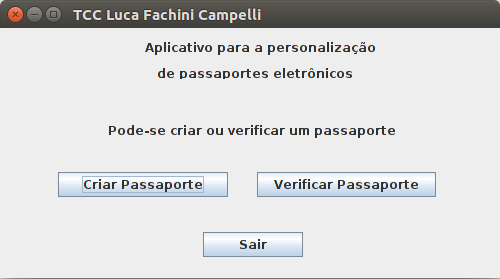
\includegraphics[width=200pt]{TelaInicial.png}
				  \caption{Tela Inicial.}
				  \label{fig:telainicial}
				\end{figure}

				\hspace*{2cm} A foto é enviada clicando-se duas vezes no espaço dedicado a ela, o que fará abrir uma janela para captura da foto. Isto ligará a primeira câmera encontrada na máquina, e com o apertar de um botão, irá retirar uma foto, que aparecerá no espaço da janela principal. Clicando no botão de digitais, a janela para coleta de digitais apareçerá. Clicando-se duas vezes no espaço a imagem de cada dedo, uma caixa de diálogo mostrará que a leitora está pronta para coleta.\footnote{Como explicado na seção de desenvolvimento, existe uma falta de comunicação entre a biblioteca em C rodando em JNI, e as Threads Java, portanto o efetivo tempo de preparo da leitora é maior do que o tempo levado para a caixa de diálogo aparecer}Ao se escanear uma digital, a sua imagem apareçerá no espaço indicado, e a caixa de diálogo se fechará automáticamente. Fazendo isso com todas as digitais, deve-se clicar no botão salvar, para que elas sejam efetivamente guardadas no cartão.\\
				Imagens Imagens Ibagens
				\hspace*{2cm} Todos os protocolos de segurança são configurados automáticamente ao se enviar as informações para o cartão: O protocolo BAC será configurado com as informações do MRZ, o protocolo PA, com certificados guardados em uma keystore na máquina e com os arquivos do cartão que estão sendo enviados, o protocolo AA terá um par de chaves gerado aleatóriamente na hora do envio.
			
			\end{justify}

	\section{Testes e Confirmações}
		\begin{justify}
			
			
		\end{justify}

\begingroup
	\section{Referências}
		\renewcommand{\section}[2]{}
		
		\printbibliography		
		
\endgroup
\end{document}
